\documentclass[twoside]{book}

% Packages required by doxygen
\usepackage{fixltx2e}
\usepackage{calc}
\usepackage{doxygen}
\usepackage[export]{adjustbox} % also loads graphicx
\usepackage{graphicx}
\usepackage[utf8]{inputenc}
\usepackage{makeidx}
\usepackage{multicol}
\usepackage{multirow}
\PassOptionsToPackage{warn}{textcomp}
\usepackage{textcomp}
\usepackage[nointegrals]{wasysym}
\usepackage[table]{xcolor}

% Font selection
\usepackage[T1]{fontenc}
\usepackage[scaled=.90]{helvet}
\usepackage{courier}
\usepackage{amssymb}
\usepackage{sectsty}
\renewcommand{\familydefault}{\sfdefault}
\allsectionsfont{%
  \fontseries{bc}\selectfont%
  \color{darkgray}%
}
\renewcommand{\DoxyLabelFont}{%
  \fontseries{bc}\selectfont%
  \color{darkgray}%
}
\newcommand{\+}{\discretionary{\mbox{\scriptsize$\hookleftarrow$}}{}{}}

% Page & text layout
\usepackage{geometry}
\geometry{%
  a4paper,%
  top=2.5cm,%
  bottom=2.5cm,%
  left=2.5cm,%
  right=2.5cm%
}
\tolerance=750
\hfuzz=15pt
\hbadness=750
\setlength{\emergencystretch}{15pt}
\setlength{\parindent}{0cm}
\setlength{\parskip}{3ex plus 2ex minus 2ex}
\makeatletter
\renewcommand{\paragraph}{%
  \@startsection{paragraph}{4}{0ex}{-1.0ex}{1.0ex}{%
    \normalfont\normalsize\bfseries\SS@parafont%
  }%
}
\renewcommand{\subparagraph}{%
  \@startsection{subparagraph}{5}{0ex}{-1.0ex}{1.0ex}{%
    \normalfont\normalsize\bfseries\SS@subparafont%
  }%
}
\makeatother

% Headers & footers
\usepackage{fancyhdr}
\pagestyle{fancyplain}
\fancyhead[LE]{\fancyplain{}{\bfseries\thepage}}
\fancyhead[CE]{\fancyplain{}{}}
\fancyhead[RE]{\fancyplain{}{\bfseries\leftmark}}
\fancyhead[LO]{\fancyplain{}{\bfseries\rightmark}}
\fancyhead[CO]{\fancyplain{}{}}
\fancyhead[RO]{\fancyplain{}{\bfseries\thepage}}
\fancyfoot[LE]{\fancyplain{}{}}
\fancyfoot[CE]{\fancyplain{}{}}
\fancyfoot[RE]{\fancyplain{}{\bfseries\scriptsize Generated by Doxygen }}
\fancyfoot[LO]{\fancyplain{}{\bfseries\scriptsize Generated by Doxygen }}
\fancyfoot[CO]{\fancyplain{}{}}
\fancyfoot[RO]{\fancyplain{}{}}
\renewcommand{\footrulewidth}{0.4pt}
\renewcommand{\chaptermark}[1]{%
  \markboth{#1}{}%
}
\renewcommand{\sectionmark}[1]{%
  \markright{\thesection\ #1}%
}

% Indices & bibliography
\usepackage{natbib}
\usepackage[titles]{tocloft}
\setcounter{tocdepth}{3}
\setcounter{secnumdepth}{5}
\makeindex

% Hyperlinks (required, but should be loaded last)
\usepackage{ifpdf}
\ifpdf
  \usepackage[pdftex,pagebackref=true]{hyperref}
\else
  \usepackage[ps2pdf,pagebackref=true]{hyperref}
\fi
\hypersetup{%
  colorlinks=true,%
  linkcolor=blue,%
  citecolor=blue,%
  unicode%
}

% Custom commands
\newcommand{\clearemptydoublepage}{%
  \newpage{\pagestyle{empty}\cleardoublepage}%
}

\usepackage{caption}
\captionsetup{labelsep=space,justification=centering,font={bf},singlelinecheck=off,skip=4pt,position=top}

%===== C O N T E N T S =====

\begin{document}

% Titlepage & ToC
\hypersetup{pageanchor=false,
             bookmarksnumbered=true,
             pdfencoding=unicode
            }
\pagenumbering{alph}
\begin{titlepage}
\vspace*{7cm}
\begin{center}%
{\Large student\+\_\+management\+\_\+sys \\[1ex]\large 1.\+0.\+0 }\\
\vspace*{1cm}
{\large Generated by Doxygen 1.8.13}\\
\end{center}
\end{titlepage}
\clearemptydoublepage
\pagenumbering{roman}
\tableofcontents
\clearemptydoublepage
\pagenumbering{arabic}
\hypersetup{pageanchor=true}

%--- Begin generated contents ---
\chapter{File Index}
\section{File List}
Here is a list of all files with brief descriptions\+:\begin{DoxyCompactList}
\item\contentsline{section}{src/\hyperlink{cmd__modes_8c}{cmd\+\_\+modes.\+c} }{\pageref{cmd__modes_8c}}{}
\item\contentsline{section}{src/\hyperlink{f__ser_8c}{f\+\_\+ser.\+c} \\*Implements functions for the string file serialization }{\pageref{f__ser_8c}}{}
\item\contentsline{section}{src/\hyperlink{main_8c}{main.\+c} \\*Implements the main function }{\pageref{main_8c}}{}
\item\contentsline{section}{src/\hyperlink{opt__proc_8c}{opt\+\_\+proc.\+c} \\*Implements functions for processing of the command line options }{\pageref{opt__proc_8c}}{}
\item\contentsline{section}{src/\hyperlink{s__manage_8c}{s\+\_\+manage.\+c} }{\pageref{s__manage_8c}}{}
\end{DoxyCompactList}

\chapter{File Documentation}
\hypertarget{cmd__modes_8c}{}\section{src/cmd\+\_\+modes.c File Reference}
\label{cmd__modes_8c}\index{src/cmd\+\_\+modes.\+c@{src/cmd\+\_\+modes.\+c}}
{\ttfamily \#include $<$stdio.\+h$>$}\newline
{\ttfamily \#include $<$stdlib.\+h$>$}\newline
{\ttfamily \#include $<$string.\+h$>$}\newline
{\ttfamily \#include \char`\"{}cmd\+\_\+modes.\+h\char`\"{}}\newline
{\ttfamily \#include \char`\"{}student.\+h\char`\"{}}\newline
{\ttfamily \#include \char`\"{}s\+\_\+manage.\+h\char`\"{}}\newline
{\ttfamily \#include \char`\"{}f\+\_\+ser.\+h\char`\"{}}\newline
Include dependency graph for cmd\+\_\+modes.\+c\+:
\nopagebreak
\begin{figure}[H]
\begin{center}
\leavevmode
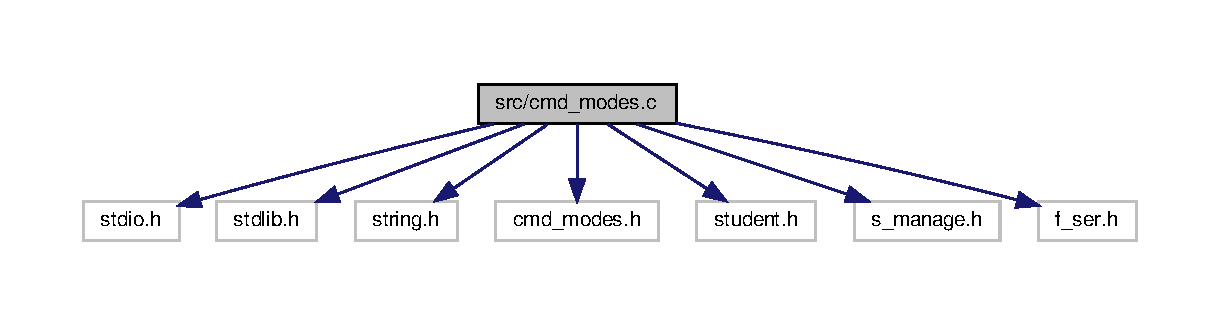
\includegraphics[width=350pt]{d2/daf/cmd__modes_8c__incl}
\end{center}
\end{figure}
\subsection*{Macros}
\begin{DoxyCompactItemize}
\item 
\#define \hyperlink{cmd__modes_8c_a5a2a76e18bbd8b8cd9026f1cee18f197}{A\+P\+P\+E\+ND}~\char`\"{}append\char`\"{}
\item 
\#define \hyperlink{cmd__modes_8c_aed0a8f83088c41d721066cd5b3b9a00c}{L\+I\+ST}~\char`\"{}list\char`\"{}
\item 
\#define \hyperlink{cmd__modes_8c_ad24e2b54375e12474e65ebf7175988fb}{Q\+U\+IT}~\char`\"{}quit\char`\"{}
\end{DoxyCompactItemize}
\subsection*{Functions}
\begin{DoxyCompactItemize}
\item 
void \hyperlink{cmd__modes_8c_a6bd3f4c41159820ee0125c2b6fd288e6}{enter\+\_\+interactive\+\_\+mode} (F\+I\+LE $\ast$fp)
\item 
void \hyperlink{cmd__modes_8c_a7660b65e581939cb0ef67b29cb152163}{enter\+\_\+append\+\_\+mode} (F\+I\+LE $\ast$fp)
\item 
void \hyperlink{cmd__modes_8c_af40fd7b8adb0868e83a057309597583f}{enter\+\_\+listing\+\_\+mode} (F\+I\+LE $\ast$fp)
\item 
void \hyperlink{cmd__modes_8c_ae6040be3d996836ef906f2bc3a359425}{start\+\_\+cmd\+\_\+mode} (F\+I\+LE $\ast$fp, char mode)
\end{DoxyCompactItemize}


\subsection{Macro Definition Documentation}
\mbox{\Hypertarget{cmd__modes_8c_a5a2a76e18bbd8b8cd9026f1cee18f197}\label{cmd__modes_8c_a5a2a76e18bbd8b8cd9026f1cee18f197}} 
\index{cmd\+\_\+modes.\+c@{cmd\+\_\+modes.\+c}!A\+P\+P\+E\+ND@{A\+P\+P\+E\+ND}}
\index{A\+P\+P\+E\+ND@{A\+P\+P\+E\+ND}!cmd\+\_\+modes.\+c@{cmd\+\_\+modes.\+c}}
\subsubsection{\texorpdfstring{A\+P\+P\+E\+ND}{APPEND}}
{\footnotesize\ttfamily \#define A\+P\+P\+E\+ND~\char`\"{}append\char`\"{}}

\mbox{\Hypertarget{cmd__modes_8c_aed0a8f83088c41d721066cd5b3b9a00c}\label{cmd__modes_8c_aed0a8f83088c41d721066cd5b3b9a00c}} 
\index{cmd\+\_\+modes.\+c@{cmd\+\_\+modes.\+c}!L\+I\+ST@{L\+I\+ST}}
\index{L\+I\+ST@{L\+I\+ST}!cmd\+\_\+modes.\+c@{cmd\+\_\+modes.\+c}}
\subsubsection{\texorpdfstring{L\+I\+ST}{LIST}}
{\footnotesize\ttfamily \#define L\+I\+ST~\char`\"{}list\char`\"{}}

\mbox{\Hypertarget{cmd__modes_8c_ad24e2b54375e12474e65ebf7175988fb}\label{cmd__modes_8c_ad24e2b54375e12474e65ebf7175988fb}} 
\index{cmd\+\_\+modes.\+c@{cmd\+\_\+modes.\+c}!Q\+U\+IT@{Q\+U\+IT}}
\index{Q\+U\+IT@{Q\+U\+IT}!cmd\+\_\+modes.\+c@{cmd\+\_\+modes.\+c}}
\subsubsection{\texorpdfstring{Q\+U\+IT}{QUIT}}
{\footnotesize\ttfamily \#define Q\+U\+IT~\char`\"{}quit\char`\"{}}



\subsection{Function Documentation}
\mbox{\Hypertarget{cmd__modes_8c_a7660b65e581939cb0ef67b29cb152163}\label{cmd__modes_8c_a7660b65e581939cb0ef67b29cb152163}} 
\index{cmd\+\_\+modes.\+c@{cmd\+\_\+modes.\+c}!enter\+\_\+append\+\_\+mode@{enter\+\_\+append\+\_\+mode}}
\index{enter\+\_\+append\+\_\+mode@{enter\+\_\+append\+\_\+mode}!cmd\+\_\+modes.\+c@{cmd\+\_\+modes.\+c}}
\subsubsection{\texorpdfstring{enter\+\_\+append\+\_\+mode()}{enter\_append\_mode()}}
{\footnotesize\ttfamily void enter\+\_\+append\+\_\+mode (\begin{DoxyParamCaption}\item[{F\+I\+LE $\ast$}]{fp }\end{DoxyParamCaption})}

\mbox{\Hypertarget{cmd__modes_8c_a6bd3f4c41159820ee0125c2b6fd288e6}\label{cmd__modes_8c_a6bd3f4c41159820ee0125c2b6fd288e6}} 
\index{cmd\+\_\+modes.\+c@{cmd\+\_\+modes.\+c}!enter\+\_\+interactive\+\_\+mode@{enter\+\_\+interactive\+\_\+mode}}
\index{enter\+\_\+interactive\+\_\+mode@{enter\+\_\+interactive\+\_\+mode}!cmd\+\_\+modes.\+c@{cmd\+\_\+modes.\+c}}
\subsubsection{\texorpdfstring{enter\+\_\+interactive\+\_\+mode()}{enter\_interactive\_mode()}}
{\footnotesize\ttfamily void enter\+\_\+interactive\+\_\+mode (\begin{DoxyParamCaption}\item[{F\+I\+LE $\ast$}]{fp }\end{DoxyParamCaption})}

\mbox{\Hypertarget{cmd__modes_8c_af40fd7b8adb0868e83a057309597583f}\label{cmd__modes_8c_af40fd7b8adb0868e83a057309597583f}} 
\index{cmd\+\_\+modes.\+c@{cmd\+\_\+modes.\+c}!enter\+\_\+listing\+\_\+mode@{enter\+\_\+listing\+\_\+mode}}
\index{enter\+\_\+listing\+\_\+mode@{enter\+\_\+listing\+\_\+mode}!cmd\+\_\+modes.\+c@{cmd\+\_\+modes.\+c}}
\subsubsection{\texorpdfstring{enter\+\_\+listing\+\_\+mode()}{enter\_listing\_mode()}}
{\footnotesize\ttfamily void enter\+\_\+listing\+\_\+mode (\begin{DoxyParamCaption}\item[{F\+I\+LE $\ast$}]{fp }\end{DoxyParamCaption})}

\mbox{\Hypertarget{cmd__modes_8c_ae6040be3d996836ef906f2bc3a359425}\label{cmd__modes_8c_ae6040be3d996836ef906f2bc3a359425}} 
\index{cmd\+\_\+modes.\+c@{cmd\+\_\+modes.\+c}!start\+\_\+cmd\+\_\+mode@{start\+\_\+cmd\+\_\+mode}}
\index{start\+\_\+cmd\+\_\+mode@{start\+\_\+cmd\+\_\+mode}!cmd\+\_\+modes.\+c@{cmd\+\_\+modes.\+c}}
\subsubsection{\texorpdfstring{start\+\_\+cmd\+\_\+mode()}{start\_cmd\_mode()}}
{\footnotesize\ttfamily void start\+\_\+cmd\+\_\+mode (\begin{DoxyParamCaption}\item[{F\+I\+LE $\ast$}]{fp,  }\item[{char}]{mode }\end{DoxyParamCaption})}


\hypertarget{f__ser_8c}{}\section{src/f\+\_\+ser.c File Reference}
\label{f__ser_8c}\index{src/f\+\_\+ser.\+c@{src/f\+\_\+ser.\+c}}


Implements functions for the string file serialization.  


{\ttfamily \#include $<$stdio.\+h$>$}\newline
{\ttfamily \#include $<$malloc.\+h$>$}\newline
{\ttfamily \#include $<$unistd.\+h$>$}\newline
{\ttfamily \#include \char`\"{}f\+\_\+ser.\+h\char`\"{}}\newline
{\ttfamily \#include \char`\"{}student.\+h\char`\"{}}\newline
Include dependency graph for f\+\_\+ser.\+c\+:
\nopagebreak
\begin{figure}[H]
\begin{center}
\leavevmode
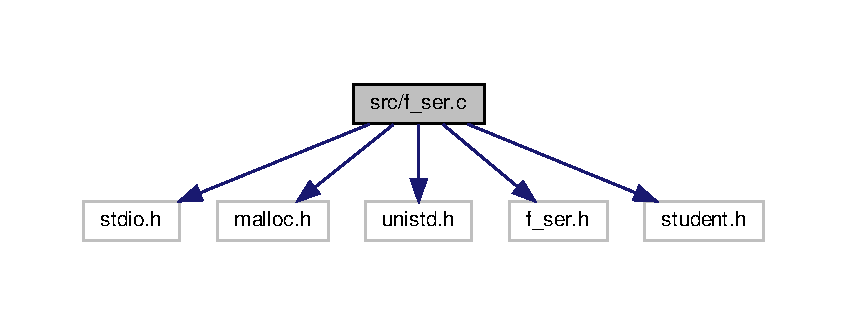
\includegraphics[width=350pt]{d4/d93/f__ser_8c__incl}
\end{center}
\end{figure}
\subsection*{Functions}
\begin{DoxyCompactItemize}
\item 
int \hyperlink{f__ser_8c_a1fe326bef22c52afabacb496673e8fa0}{str\+\_\+len} (const char $\ast$str)
\begin{DoxyCompactList}\small\item\em Returns the number of characters in a given string. \end{DoxyCompactList}\item 
int \hyperlink{f__ser_8c_a7c45394872b4d2ed8a03ae2410d73f8c}{student\+\_\+write} (F\+I\+LE $\ast$fp, student\+\_\+t student)
\begin{DoxyCompactList}\small\item\em Writes an input string into the file. \end{DoxyCompactList}\item 
int \hyperlink{f__ser_8c_a59f58841a59c7aacc0741afd75296f75}{student\+\_\+read} (F\+I\+LE $\ast$fp)
\begin{DoxyCompactList}\small\item\em Reads a string from the file. \end{DoxyCompactList}\end{DoxyCompactItemize}


\subsection{Detailed Description}
Implements functions for the string file serialization. 

Copyright (C) 2003-\/2019 Dipl.\+Ing. Dr. techn. Idriz Smaili. All rights reserved Siebenbuergerstrasse 16-\/26/26/17, A--1220 Wien, Austria. \href{mailto:smaili.idriz@gmail.com}{\tt smaili.\+idriz@gmail.\+com}

\begin{DoxyAuthor}{Author}
(IS) Dr.\+techn. Dipl.-\/\+Ing. Idriz Smaili (\href{mailto:smaili.idriz@gmail.com}{\tt smaili.\+idriz@gmail.\+com}) 
\end{DoxyAuthor}
\begin{DoxyDate}{Date}

\end{DoxyDate}
\begin{DoxyParagraph}{Date}
Fri Apr 20, 15\+:27\+:59 W\+E\+ST 2019 
\end{DoxyParagraph}


\subsection{Function Documentation}
\mbox{\Hypertarget{f__ser_8c_a1fe326bef22c52afabacb496673e8fa0}\label{f__ser_8c_a1fe326bef22c52afabacb496673e8fa0}} 
\index{f\+\_\+ser.\+c@{f\+\_\+ser.\+c}!str\+\_\+len@{str\+\_\+len}}
\index{str\+\_\+len@{str\+\_\+len}!f\+\_\+ser.\+c@{f\+\_\+ser.\+c}}
\subsubsection{\texorpdfstring{str\+\_\+len()}{str\_len()}}
{\footnotesize\ttfamily int str\+\_\+len (\begin{DoxyParamCaption}\item[{const char $\ast$}]{str }\end{DoxyParamCaption})}



Returns the number of characters in a given string. 


\begin{DoxyParams}[1]{Parameters}
\mbox{\tt in}  & {\em input} & string\\
\hline
\end{DoxyParams}

\begin{DoxyRetVals}{Return values}
{\em number} & of characters \\
\hline
\end{DoxyRetVals}
\mbox{\Hypertarget{f__ser_8c_a59f58841a59c7aacc0741afd75296f75}\label{f__ser_8c_a59f58841a59c7aacc0741afd75296f75}} 
\index{f\+\_\+ser.\+c@{f\+\_\+ser.\+c}!student\+\_\+read@{student\+\_\+read}}
\index{student\+\_\+read@{student\+\_\+read}!f\+\_\+ser.\+c@{f\+\_\+ser.\+c}}
\subsubsection{\texorpdfstring{student\+\_\+read()}{student\_read()}}
{\footnotesize\ttfamily int student\+\_\+read (\begin{DoxyParamCaption}\item[{F\+I\+LE $\ast$}]{fp }\end{DoxyParamCaption})}



Reads a string from the file. 

First the four (4) bytes will be read, which indicate the length of the string to be read, and then the string itself will be read.


\begin{DoxyParams}[1]{Parameters}
\mbox{\tt in,out}  & {\em fp} & -\/ file pointer \\
\hline
\mbox{\tt out}  & {\em dst} & -\/ pointer to the newly allocated string\\
\hline
\end{DoxyParams}

\begin{DoxyRetVals}{Return values}
{\em 0} & in case an error was occured \\
\hline
{\em -\/1} & error allocating memory was occured \\
\hline
{\em $>$0} & number of bytes written in the file \\
\hline
\end{DoxyRetVals}
\mbox{\Hypertarget{f__ser_8c_a7c45394872b4d2ed8a03ae2410d73f8c}\label{f__ser_8c_a7c45394872b4d2ed8a03ae2410d73f8c}} 
\index{f\+\_\+ser.\+c@{f\+\_\+ser.\+c}!student\+\_\+write@{student\+\_\+write}}
\index{student\+\_\+write@{student\+\_\+write}!f\+\_\+ser.\+c@{f\+\_\+ser.\+c}}
\subsubsection{\texorpdfstring{student\+\_\+write()}{student\_write()}}
{\footnotesize\ttfamily int student\+\_\+write (\begin{DoxyParamCaption}\item[{F\+I\+LE $\ast$}]{fp,  }\item[{student\+\_\+t}]{student }\end{DoxyParamCaption})}



Writes an input string into the file. 

First the four (4) bytes will be written indicating the length of the string to be written, and then the string itself will be written.


\begin{DoxyParams}[1]{Parameters}
\mbox{\tt in,out}  & {\em fp} & -\/ file pointer \\
\hline
\mbox{\tt in}  & {\em str} & -\/ the input string\\
\hline
\end{DoxyParams}

\begin{DoxyRetVals}{Return values}
{\em 0} & in case an error was occured \\
\hline
{\em $>$0} & number of bytes written in the file \\
\hline
\end{DoxyRetVals}

\hypertarget{main_8c}{}\section{src/main.c File Reference}
\label{main_8c}\index{src/main.\+c@{src/main.\+c}}


Implements the main function.  


{\ttfamily \#include $<$stdio.\+h$>$}\newline
{\ttfamily \#include $<$stdlib.\+h$>$}\newline
{\ttfamily \#include $<$errno.\+h$>$}\newline
{\ttfamily \#include $<$string.\+h$>$}\newline
{\ttfamily \#include $<$signal.\+h$>$}\newline
{\ttfamily \#include \char`\"{}opt\+\_\+proc.\+h\char`\"{}}\newline
{\ttfamily \#include \char`\"{}cmd\+\_\+modes.\+h\char`\"{}}\newline
Include dependency graph for main.\+c\+:
\nopagebreak
\begin{figure}[H]
\begin{center}
\leavevmode
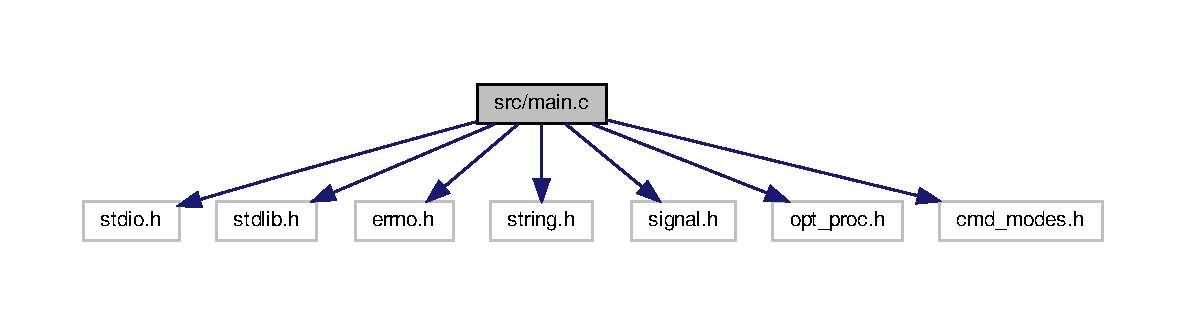
\includegraphics[width=350pt]{d4/d10/main_8c__incl}
\end{center}
\end{figure}
\subsection*{Functions}
\begin{DoxyCompactItemize}
\item 
int \hyperlink{main_8c_a0ddf1224851353fc92bfbff6f499fa97}{main} (int argc, char $\ast$argv\mbox{[}$\,$\mbox{]})
\end{DoxyCompactItemize}


\subsection{Detailed Description}
Implements the main function. 

Copyright (C) 2019 Bsc. Armend Ukehaxhaj. All rights reserved Rr. Agim Ramadani pn., Prishtine, Kosovo. \href{mailto:armendd.u@hotmail.com}{\tt armendd.\+u@hotmail.\+com}

\begin{DoxyAuthor}{Author}
(IS) Bsc. Armend Ukehaxhaj (\href{mailto:armendd.u@hotmail.com}{\tt armendd.\+u@hotmail.\+com}) 
\end{DoxyAuthor}
\begin{DoxyDate}{Date}

\end{DoxyDate}
\begin{DoxyParagraph}{Date}
19 May 19, 18\+:20\+:52 W\+E\+ST 2019 
\end{DoxyParagraph}


\subsection{Function Documentation}
\mbox{\Hypertarget{main_8c_a0ddf1224851353fc92bfbff6f499fa97}\label{main_8c_a0ddf1224851353fc92bfbff6f499fa97}} 
\index{main.\+c@{main.\+c}!main@{main}}
\index{main@{main}!main.\+c@{main.\+c}}
\subsubsection{\texorpdfstring{main()}{main()}}
{\footnotesize\ttfamily int main (\begin{DoxyParamCaption}\item[{int}]{argc,  }\item[{char $\ast$}]{argv\mbox{[}$\,$\mbox{]} }\end{DoxyParamCaption})}


\hypertarget{opt__proc_8c}{}\section{src/opt\+\_\+proc.c File Reference}
\label{opt__proc_8c}\index{src/opt\+\_\+proc.\+c@{src/opt\+\_\+proc.\+c}}


Implements functions for processing of the command line options.  


{\ttfamily \#include $<$stdio.\+h$>$}\newline
{\ttfamily \#include $<$stdlib.\+h$>$}\newline
{\ttfamily \#include $<$unistd.\+h$>$}\newline
{\ttfamily \#include $<$getopt.\+h$>$}\newline
{\ttfamily \#include $<$signal.\+h$>$}\newline
{\ttfamily \#include \char`\"{}opt\+\_\+proc.\+h\char`\"{}}\newline
Include dependency graph for opt\+\_\+proc.\+c\+:
\nopagebreak
\begin{figure}[H]
\begin{center}
\leavevmode
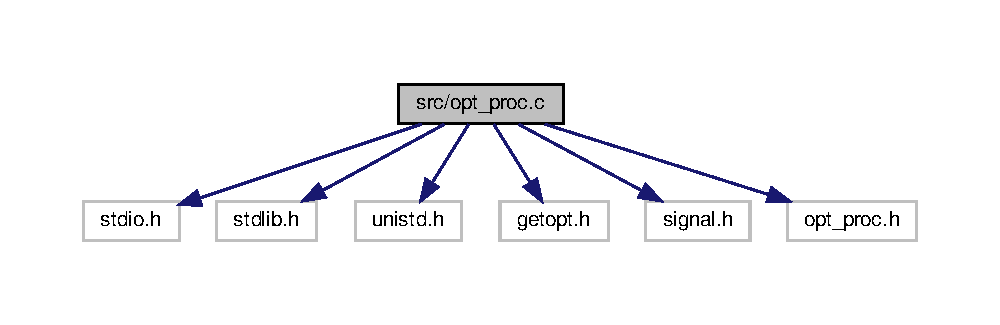
\includegraphics[width=350pt]{d7/d2c/opt__proc_8c__incl}
\end{center}
\end{figure}
\subsection*{Functions}
\begin{DoxyCompactItemize}
\item 
void \hyperlink{opt__proc_8c_ae1d706d7c4ba99ef535a1a7cede59a38}{usage} (const char $\ast$app\+\_\+name)
\item 
char \hyperlink{opt__proc_8c_a123cebbebdf6a4997ac1e34c643b51ad}{set\+\_\+mode} (int argc, char $\ast$$\ast$argv, char $\ast$$\ast$f\+\_\+name)
\item 
void \hyperlink{opt__proc_8c_af9df740ebf79d2e8f7e3718c0c0986b4}{handle\+\_\+sigint} (int sig\+\_\+num)
\end{DoxyCompactItemize}


\subsection{Detailed Description}
Implements functions for processing of the command line options. 

Copyright (C) 2019 Bsc. Armend Ukehaxhaj. All rights reserved Rr. Agim Ramadani pn., Prishtine, Kosovo. \href{mailto:armendd.u@hotmail.com}{\tt armendd.\+u@hotmail.\+com}

\begin{DoxyAuthor}{Author}
(IS) Bsc. Armend Ukehaxhaj (\href{mailto:armendd.u@hotmail.com}{\tt armendd.\+u@hotmail.\+com}) 
\end{DoxyAuthor}
\begin{DoxyDate}{Date}

\end{DoxyDate}
\begin{DoxyParagraph}{Date}
19 May 19, 18\+:20\+:52 W\+E\+ST 2019 
\end{DoxyParagraph}


\subsection{Function Documentation}
\mbox{\Hypertarget{opt__proc_8c_af9df740ebf79d2e8f7e3718c0c0986b4}\label{opt__proc_8c_af9df740ebf79d2e8f7e3718c0c0986b4}} 
\index{opt\+\_\+proc.\+c@{opt\+\_\+proc.\+c}!handle\+\_\+sigint@{handle\+\_\+sigint}}
\index{handle\+\_\+sigint@{handle\+\_\+sigint}!opt\+\_\+proc.\+c@{opt\+\_\+proc.\+c}}
\subsubsection{\texorpdfstring{handle\+\_\+sigint()}{handle\_sigint()}}
{\footnotesize\ttfamily void handle\+\_\+sigint (\begin{DoxyParamCaption}\item[{int}]{sig\+\_\+num }\end{DoxyParamCaption})}

\mbox{\Hypertarget{opt__proc_8c_a123cebbebdf6a4997ac1e34c643b51ad}\label{opt__proc_8c_a123cebbebdf6a4997ac1e34c643b51ad}} 
\index{opt\+\_\+proc.\+c@{opt\+\_\+proc.\+c}!set\+\_\+mode@{set\+\_\+mode}}
\index{set\+\_\+mode@{set\+\_\+mode}!opt\+\_\+proc.\+c@{opt\+\_\+proc.\+c}}
\subsubsection{\texorpdfstring{set\+\_\+mode()}{set\_mode()}}
{\footnotesize\ttfamily char set\+\_\+mode (\begin{DoxyParamCaption}\item[{int}]{argc,  }\item[{char $\ast$$\ast$}]{argv,  }\item[{char $\ast$$\ast$}]{f\+\_\+name }\end{DoxyParamCaption})}

\mbox{\Hypertarget{opt__proc_8c_ae1d706d7c4ba99ef535a1a7cede59a38}\label{opt__proc_8c_ae1d706d7c4ba99ef535a1a7cede59a38}} 
\index{opt\+\_\+proc.\+c@{opt\+\_\+proc.\+c}!usage@{usage}}
\index{usage@{usage}!opt\+\_\+proc.\+c@{opt\+\_\+proc.\+c}}
\subsubsection{\texorpdfstring{usage()}{usage()}}
{\footnotesize\ttfamily void usage (\begin{DoxyParamCaption}\item[{const char $\ast$}]{app\+\_\+name }\end{DoxyParamCaption})}


\hypertarget{s__manage_8c}{}\section{src/s\+\_\+manage.c File Reference}
\label{s__manage_8c}\index{src/s\+\_\+manage.\+c@{src/s\+\_\+manage.\+c}}
{\ttfamily \#include $<$stdlib.\+h$>$}\newline
{\ttfamily \#include $<$stdio.\+h$>$}\newline
{\ttfamily \#include $<$string.\+h$>$}\newline
{\ttfamily \#include \char`\"{}s\+\_\+manage.\+h\char`\"{}}\newline
{\ttfamily \#include \char`\"{}f\+\_\+ser.\+h\char`\"{}}\newline
Include dependency graph for s\+\_\+manage.\+c\+:
\nopagebreak
\begin{figure}[H]
\begin{center}
\leavevmode
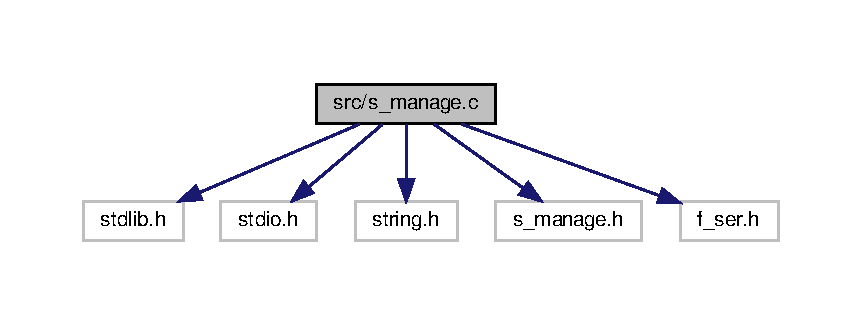
\includegraphics[width=350pt]{d3/dfe/s__manage_8c__incl}
\end{center}
\end{figure}
\subsection*{Functions}
\begin{DoxyCompactItemize}
\item 
void \hyperlink{s__manage_8c_af59fb0dbb47bc751c920d0c10a5be205}{get\+\_\+student\+\_\+info} (student\+\_\+t $\ast$s)
\item 
int \hyperlink{s__manage_8c_a9273350f161ec20f7c10b53e3363f73b}{get\+\_\+no\+\_\+students} (F\+I\+LE $\ast$fp)
\end{DoxyCompactItemize}


\subsection{Function Documentation}
\mbox{\Hypertarget{s__manage_8c_a9273350f161ec20f7c10b53e3363f73b}\label{s__manage_8c_a9273350f161ec20f7c10b53e3363f73b}} 
\index{s\+\_\+manage.\+c@{s\+\_\+manage.\+c}!get\+\_\+no\+\_\+students@{get\+\_\+no\+\_\+students}}
\index{get\+\_\+no\+\_\+students@{get\+\_\+no\+\_\+students}!s\+\_\+manage.\+c@{s\+\_\+manage.\+c}}
\subsubsection{\texorpdfstring{get\+\_\+no\+\_\+students()}{get\_no\_students()}}
{\footnotesize\ttfamily int get\+\_\+no\+\_\+students (\begin{DoxyParamCaption}\item[{F\+I\+LE $\ast$}]{fp }\end{DoxyParamCaption})}

\mbox{\Hypertarget{s__manage_8c_af59fb0dbb47bc751c920d0c10a5be205}\label{s__manage_8c_af59fb0dbb47bc751c920d0c10a5be205}} 
\index{s\+\_\+manage.\+c@{s\+\_\+manage.\+c}!get\+\_\+student\+\_\+info@{get\+\_\+student\+\_\+info}}
\index{get\+\_\+student\+\_\+info@{get\+\_\+student\+\_\+info}!s\+\_\+manage.\+c@{s\+\_\+manage.\+c}}
\subsubsection{\texorpdfstring{get\+\_\+student\+\_\+info()}{get\_student\_info()}}
{\footnotesize\ttfamily void get\+\_\+student\+\_\+info (\begin{DoxyParamCaption}\item[{student\+\_\+t $\ast$}]{s }\end{DoxyParamCaption})}


%--- End generated contents ---

% Index
\backmatter
\newpage
\phantomsection
\clearemptydoublepage
\addcontentsline{toc}{chapter}{Index}
\printindex

\end{document}
